% Part II report (Deliverable II.4) on a Continuous Page. Build it with ./build.sh, which first generates
% generated/*.tex from the code and from CI; latexmk -lualatex report_2.tex alone reuses the committed ones.
\documentclass{article}

\usepackage[textwidth=16cm, sidenotes=false, variablewidth=true, backref=true]{continuous-page}

\usepackage[english]{babel}
\usepackage{csquotes}
\usepackage{microtype}
\usepackage{booktabs}
\usepackage{tabularx}
\usepackage{caption}
\usepackage{enumitem}
\usepackage{fancyvrb}
\usepackage{tikz}
\usetikzlibrary{positioning, graphdrawing, arrows.meta, quotes}
\usegdlibrary{layered}
% BibTeX, not biber: TeX Live 2026's universal biber cannot unpack itself where lipo lacks -extract_family.
\usepackage[style=numeric, backend=bibtex]{biblatex}
\addbibresource{references.bib}
\renewcommand*{\multicitedelim}{\addsemicolon\space} % a locator's commas would blur citations together
\usepackage[pdfusetitle,hidelinks]{hyperref}
\usepackage[capitalise]{cleveref}
\usepackage{term} % \term{batches}: a glossary term, linked to its entry

% \placeholder{<who it waits on>}{<what is missing>}{<notes>}: a coloured box where content is still
% missing. Each is logged as "Placeholder: ...", so that ./build.sh final fails while any remains.
\NewDocumentCommand{\placeholder}{m m +m}{%
	\typeout{Placeholder: #2 (waits on #1)}%
	\par\smallskip\noindent\fcolorbox{orange}{orange!8}{\parbox{\dimexpr\linewidth-2\fboxsep-2\fboxrule}{%
		\small\textbf{Missing: #2.} Waits on #1.\par #3}}\par\smallskip}

% The Okabe-Ito palette, safe for colour-blind readers: every figure takes its colours from here.
\definecolor{oiorange}{HTML}{E69F00}
\definecolor{oisky}{HTML}{56B4E9}
\definecolor{oigreen}{HTML}{009E73}
\definecolor{oivermillion}{HTML}{D55E00}
\definecolor{oiblue}{HTML}{0072B2}
\definecolor{oigrey}{HTML}{999999}

% The metamodel diagrams of generated/metamodel-*.tex, of both chains.
\tikzset{
	metamodel/.style={layered layout, level sep=1.2cm, sibling sep=1.8cm},
	class/.style={draw, inner sep=0pt, font=\footnotesize},
	contain/.style={{Diamond[]}-},
	reference/.style={-{Straight Barb[]}, minimum layers=0}, % may join classes of one layer
	association/.style={-},
	role/.style={font=\scriptsize, auto, pos=0.6},
	source role/.style={font=\scriptsize, auto, pos=0.2}, % the two ends of a B-UML association
	target role/.style={font=\scriptsize, auto, pos=0.8},
}

\title{Exam-Slot Assignment with QAOA and Simulated Annealing: Part~II}
\author{Group G3: Alef Keuffer, Diogo Ferreira, Luis Arruda}
\date{\today}

\begin{document}

\maketitle

\section{Introduction}\label{sec:introduction}

Our group was assigned the exam-slot assignment problem, which describes the process of scheduling \term{exams}
within a given number of \term{batches} while avoiding conflicts, a conflict being a \term{student} having to attend
several \term{exams} that take place in the same \term{batch}.

\paragraph{Inspiration.}
At the start, we struggled to understand the problem's context and how to formulate it. Afterwards, we found a
very useful paper that deals with the same problem as ours, \enquote{Hybrid quantum annealing for large-scale exam
scheduling} \cite{Paper}. We based the output of our model-to-text transformations on it: the generated scripts of
both chains solve a \term{QUBO} over the paper's \term{assignment variables} \cite[§5.3, Eq. (4)]{Paper}, the BESSER
chain's in the paper's formulation, the EMF chain's in a weighted variant of it (\cref{app:formulation}). It helped us
formulate the problem and its constraints. Our solutions were heavily inspired by the way the paper framed
the problem: transforming students' course registrations into a course conflict matrix \cite[§5.2]{Paper}, which
the EMF chain models as a \term{Conflict Graph}.

\paragraph{Strategy.}
We decided to implement two chains, one using BESSER and one using EMF, to compare the two technologies and to get
the whole team familiar with the problem and the implementation process. More details on the chains can be found
in \cref{sec:besser,sec:emf}.

The EMF chain's terms are those of the glossary (\cref{app:glossary}); the BESSER chain's sections keep its
own words: \emph{slot} for a \term{Batch}, \emph{valid} for a \term{schedule} that places every \term{exam} without a \term{Conflict}.

\begin{figure}
	\begin{tikzpicture}[node distance=6mm and 7mm, >={Stealth[]},
			stage/.style={draw, rounded corners, align=center, text width=2.9cm, font=\small, inner sep=4pt},
			flow/.style={font=\scriptsize, midway}]
		\node[stage] (problem) {\textbf{\term{Problem}}\\\footnotesize \term{students}, \term{exams} and their \term{weights}, \term{batches}};
		\node[stage, right=of problem] (qubo) {\textbf{\term{QUBO}}\\\footnotesize an \term{Assignment Variable} per
			\term{exam} and \term{batch}, a penalty per \term{Constraint}};
		\node[stage, right=of qubo] (method) {\textbf{\term{Method}}\\\footnotesize QAOA on a simulator, or
			\term{simulated annealing} (EMF)};
		\node[stage, right=of method] (schedule) {\textbf{\term{Schedule}}\\\footnotesize a sample, decoded};
		\node[stage, below=of qubo] (baseline) {\textbf{\term{Baseline}}\\\footnotesize every \term{schedule}
			enumerated: the optimum};
		\node[stage, right=of baseline] (validation) {\textbf{Validation}\\\footnotesize \term{P(optimal)} and
			\term{P(feasible)} against chance};
		\draw[->] (problem) -- (qubo);
		\draw[->] (qubo) -- (method);
		\draw[->] (method) -- (schedule);
		\draw[->] (problem) |- (baseline);
		\draw[->] (baseline) -- (validation);
		\draw[->] (method) -- node[flow, right] {every sample} (validation);
		\draw[->] (schedule) |- node[flow, pos=0.25, right] {feasible? optimal?} (validation);
	\end{tikzpicture}
	\caption{The strategy of both chains: model the \term{Problem}, formulate it as a \term{QUBO}, sample it by a
		\term{Method}, decode a sample into a \term{Schedule}, and judge every sample against a \term{Baseline}
		that enumerates every \term{schedule}.}\label{fig:strategy}
\end{figure}

\subsection{Two chains}\label{sec:two-chains}

The strategy is implemented twice, independently: the EMF chain in \texttt{emf/}, with Xtext, ATL and Acceleo
(\cref{sec:emf}), and the BESSER chain in \texttt{besser/}, with Python transformations over B-UML models and
BESSER's Qiskit generator (\cref{sec:besser}). They solve the two formulations of \cref{app:formulation}, so only the EMF chain's
results depend on the \term{Weight}.

\begin{figure}
	\begin{tikzpicture}[
			exam/.style={circle, draw, thick, minimum size=1.55cm, align=center, font=\footnotesize, inner sep=1pt},
			conflict/.style={draw=black!40},
			broken/.style={draw=oivermillion, line width=2pt},
			b1/.style={exam, fill=oiorange!60}, b2/.style={exam, fill=oisky!60}, b3/.style={exam, fill=oigreen!60},
			unscheduled/.style={exam, dashed, draw=oigrey, text=oigrey, fill=white}]
		\begin{scope}
			\node[b1] (a) at (0, 2.2) {Algebra\\4};
			\node[b2] (c) at (2.2, 2.2) {Calculus\\3};
			\node[b3] (p) at (0, 0) {Physics\\2};
			\node[b3] (s) at (2.2, 0) {Statistics\\1};
			\draw[conflict] (a) -- (c) (a) -- (p) (a) -- (s) (c) -- (p) (c) -- (s);
			\draw[broken] (p) -- (s);
			\node[font=\small, align=center] at (1.1, -1.4) {paper's formulation:\\every \term{exam} placed, one \term{Conflict}};
		\end{scope}
		\begin{scope}[xshift=5.5cm]
			\node[b1] (a) at (0, 2.2) {Algebra\\4};
			\node[b2] (c) at (2.2, 2.2) {Calculus\\3};
			\node[b3] (p) at (0, 0) {Physics\\2};
			\node[unscheduled] (s) at (2.2, 0) {Statistics\\1};
			\draw[conflict] (a) -- (c) (a) -- (p) (c) -- (p);
			\draw[conflict, dashed, draw=oigrey] (a) -- (s) (c) -- (s) (p) -- (s);
			\node[font=\small, align=center] at (1.1, -1.4) {weighted formulation:\\Statistics an \term{Unscheduled Exam}, \term{Cost}~1};
		\end{scope}
		\begin{scope}[xshift=10.4cm, yshift=1.6cm, every node/.style={font=\footnotesize, anchor=west}]
			\node[draw, fill=oiorange!60, minimum size=3mm, label={[font=\footnotesize]right:\term{batch} 1}] at (0, 0) {};
			\node[draw, fill=oisky!60, minimum size=3mm, label={[font=\footnotesize]right:\term{batch} 2}] at (0, -0.5) {};
			\node[draw, fill=oigreen!60, minimum size=3mm, label={[font=\footnotesize]right:\term{batch} 3}] at (0, -1) {};
			\draw[broken] (0, -1.5) -- (0.4, -1.5) node[right] {broken \term{Conflict}};
		\end{scope}
	\end{tikzpicture}
	\caption{The two formulations' optima on \texttt{clique}: four \term{exams}, with their \term{weights}, that all
		share every \term{student}, in three \term{batches}. A node's colour is its \term{batch}; an edge, a
		\term{Conflict}. The paper's formulation places every \term{exam} and breaks one \term{Conflict}, any two
		\term{exams} sharing a \term{batch} at the same energy; the weighted one leaves the lightest \term{exam},
		Statistics, an \term{Unscheduled Exam}, at \term{Cost}~1.}\label{fig:clique}
\end{figure}


% Section: EMF chain map. \input by report_2.tex. Detail in app:emf.
\section{EMF chain}\label{sec:emf}

\paragraph{One problem, followed end to end.}
Take the smallest instance, \texttt{emf/instances/1-path.exam}: four exams whose conflicts form a path,
two batches.

\VerbatimInput[fontsize=\footnotesize, frame=topline, label=\texttt{1-path.exam}]{../../emf/instances/1-path.exam}

Running \texttt{cd emf \&\& ./build.sh} turns that text into the files in \texttt{emf/out/path/}. What
happens to it, in order:

\begin{enumerate}[nosep, leftmargin=*]
	\item \texttt{1-path.exam} (text).
	\item Xtext: the parser from \texttt{Exam.xtext} (text~$\to$~model) yields \texttt{problem.xmi} and
	      \texttt{solverconfig.xmi}, which conform to \texttt{problem.ecore} and \texttt{solverconfig.ecore}.
	\item OCL validation, then ATL \texttt{problem2conflictgraph.atl} (model~$\to$~model) yields
	      \texttt{conflictgraph.xmi}, which conforms to \texttt{conflictgraph.ecore}.
	\item OCL validation, then Acceleo \texttt{main.mtl} (model~$\to$~text) yields
	      \texttt{solve\_path.py}.
	\item Python at run time: pyqubo builds the QUBO, then QAOA or annealing samples it, writing
	      \texttt{schedule\_path.xmi} and a printed report; the schedule conforms to \texttt{schedule.ecore}.
\end{enumerate}

The Java that glues the first three arrows is one class,
\texttt{ChainApplication.java} in the chain bundle
(\path{emf/bundles/pt.up.feup.examschedule.chain/}). Its \texttt{run} method is the chain above: parse,
validate, save, ATL, save, validate, Acceleo. The grammar, ATL module, Acceleo template and runtime are
expanded in \cref{app:emf}.

\paragraph{Three metalevels.}
Each \texttt{.xmi} file is a \emph{model}. It is only meaningful because it \emph{conforms to} a
\emph{metamodel}, an \texttt{.ecore} file, which in turn is written in Ecore, EMF's metamodelling language;
XMI is how EMF serialises those models.

\begin{center}
	\small
	\begin{tabular}{@{}lll@{}}
		\toprule
		Level & In this repo & Says \\
		\midrule
		Meta-metamodel & Ecore itself & there are classes, attributes, references \\
		Metamodel & \texttt{problem.ecore} & a Problem has exams; an Exam has students \\
		Model & \texttt{emf/out/path/problem.xmi} & Calculus is sat by Ana and Rui \\
		\bottomrule
	\end{tabular}
\end{center}

The OCL constraints (\texttt{uniqueExamNames}, \texttt{atLeastOneBatch},\ldots) live \emph{inside} the
metamodel as annotations, so they travel with it and every tool that loads \texttt{problem.ecore} can check
them (\cref{app:metamodels}).

\paragraph{Three kinds of arrow.}
Model-driven engineering names transformations by what goes in and out. The chain has one of each:

\begin{itemize}[nosep]
	\item \textbf{Text~$\to$~model}: Xtext. The grammar does not invent its own classes; its rules say
	      \texttt{returns problem::Problem}, so the parser builds instances of the hand-written metamodel.
	\item \textbf{Model~$\to$~model}: ATL. Rules map a Problem to a Conflict Graph and add an edge for each
	      pair of exams sharing a student, the paper's Algorithm~1 \cite[§5.2, Algorithm 1]{Paper}.
	\item \textbf{Model~$\to$~text}: Acceleo. A template walks the Conflict Graph and prints Python.
\end{itemize}

The last model the chain itself produces is the Conflict Graph. The QUBO never becomes an \texttt{.xmi}:
pyqubo builds it in memory when the generated script runs (\texttt{emf/docs/adr/0007}), the hand-off chosen
in \cref{sec:strategy}.


% Section 3, the BESSER chain: \input by report_2.tex, so that editing it never conflicts with the rest.

In one sentence: the BESSER chain takes a description of the exams, turns it step by step into a quantum
circuit, runs that circuit on a simulator, and turns the answers back into a timetable that a person can read.
Every step reads a model and writes a model, and every model it writes is saved in
\texttt{besser/output/<instance>/}, so each step can be opened and checked on its own.
\Cref{fig:besser-chain} follows the smallest example, \texttt{tiny} (3 exams, 3 time slots, 9 qubits).

\begin{figure}
	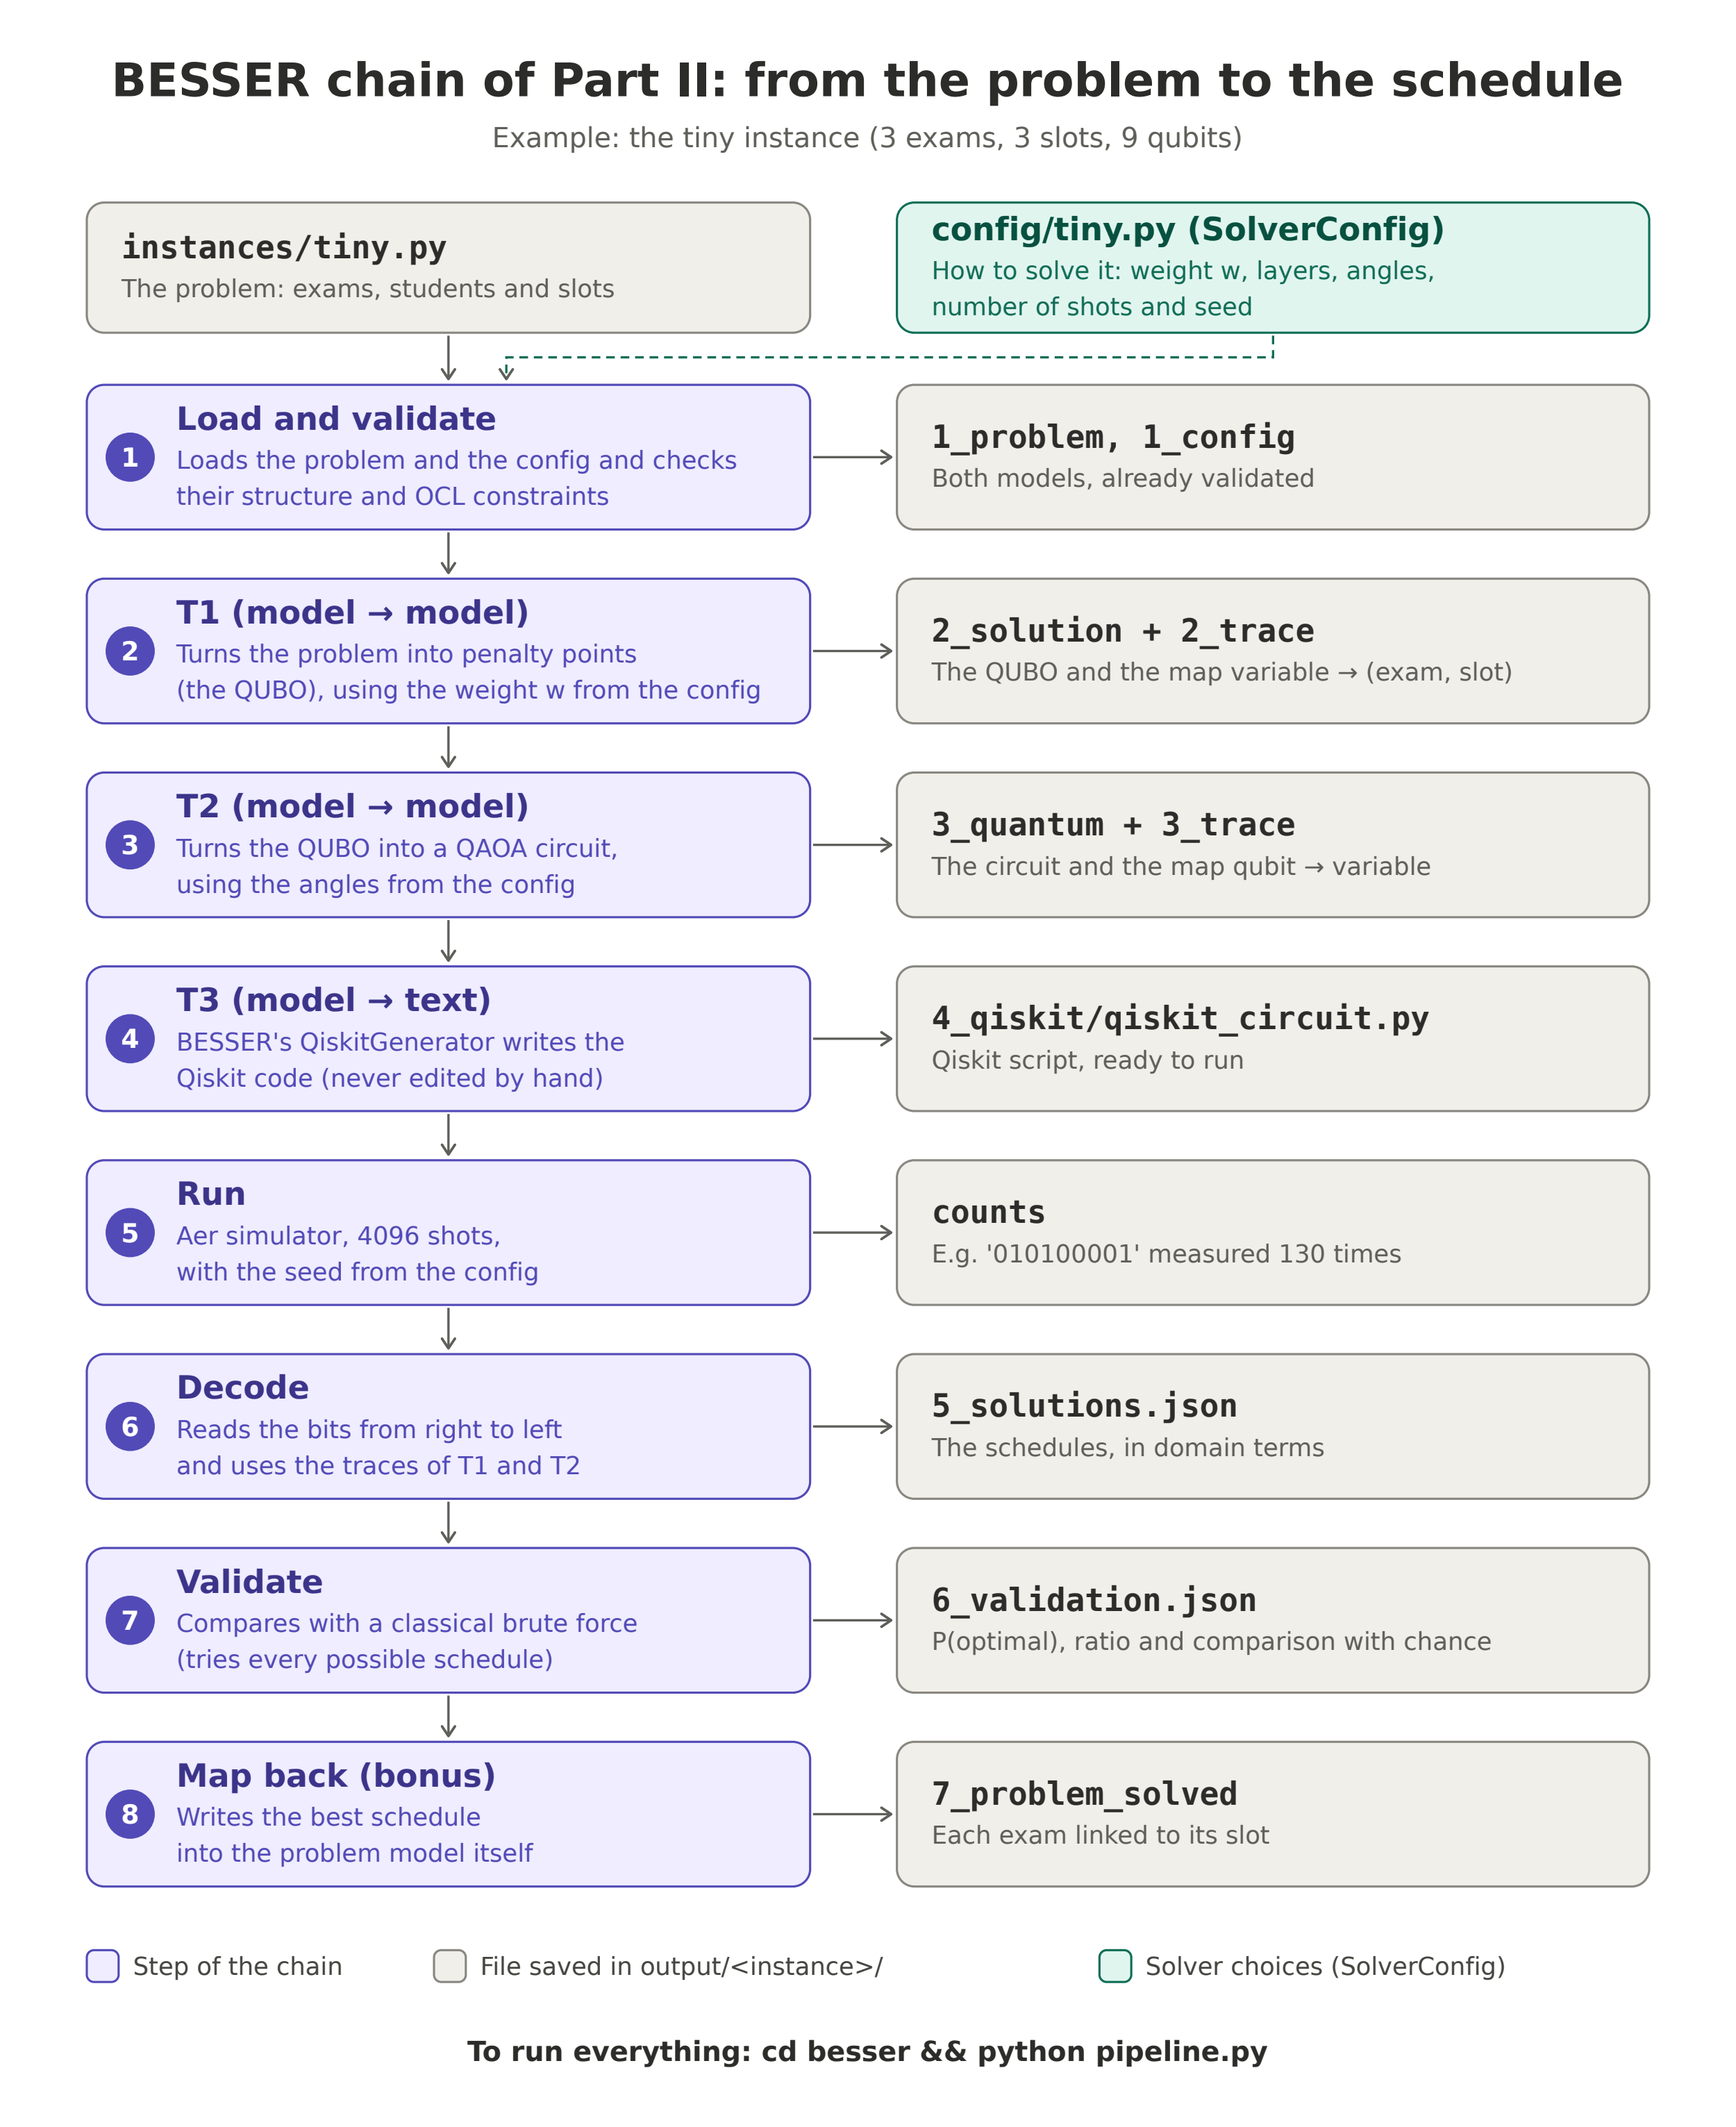
\includegraphics[width=\linewidth]{../imgs/cadeia_besser-1.png}
	\caption{The BESSER chain on the \texttt{tiny} instance: each step (left) and the model it saves (right).}
	\label{fig:besser-chain}
\end{figure}

\paragraph{Two inputs: the \emph{what} and the \emph{how}.}
Everything starts from two files written by a person. The first describes \emph{the problem}: the exams,
the students who sit them, and the time slots (\texttt{instances/tiny.py}, a model of Part~I's Problem
DSL). The second says \emph{how to solve it}: how much a conflict costs, how many layers the circuit has,
its angles, how many times to run it, and a seed so that every run gives the same result
(\texttt{config/tiny.py}, a model of our Solver Configuration metamodel). They are kept apart on purpose:
to solve the same problem in another way, only the configuration changes, never the code.

\begin{enumerate}
	\item \textbf{Read and check.} Both models are loaded and checked against the rules of their
	      metamodels, written in OCL: for example, an exam must have a name, and the number of circuit
	      layers must match the depth. If a rule fails, the chain stops here.
	      Saved: \texttt{1\_problem}, \texttt{1\_config}.
	\item \textbf{T1, model to model: from exams to penalty points.} The problem becomes a QUBO, a list of
	      penalty points. There is one yes/no variable for each pair (exam, slot), and a schedule earns
	      points for every rule it breaks: an exam with no slot or with two slots, or two exams that share a
	      student placed in the same slot \cite[§5.3]{Paper}. A schedule with zero points is a valid one.
	      Leaving an exam out always costs more than a conflict, so the solver cannot ``cheat'' by dropping
	      an exam \cite[§2.3]{Lucas}. Saved: \texttt{2\_solution}, and a trace from each variable to its
	      exam and slot.
	\item \textbf{T2, model to model: from penalty points to a quantum circuit.} The QUBO becomes a QAOA
	      circuit \cite{Farhi} in BESSER's own quantum metamodel: one qubit per variable, and layers that
	      push the qubits towards the schedules with fewer points. The angles of each layer come from the
	      configuration. Saved: \texttt{3\_quantum}, and a trace from each qubit to its variable.
	\item \textbf{T3, model to text: writing the code.} BESSER's \texttt{QiskitGenerator} writes the
	      circuit as a Qiskit script, \texttt{4\_qiskit/qiskit\_circuit.py}. The generated code is never
	      edited by hand: if something is wrong, the model or the transformation is fixed.
	\item \textbf{Run.} The script runs on the Qiskit Aer simulator \cite{Qiskit} 4096 times, with the
	      seed of the configuration. The result is a count of how often each string of bits came out.
	\item \textbf{Decode.} Each string of bits is read from right to left, as Qiskit writes it, and the two
	      traces turn every bit back into ``exam X in slot Y''. Saved: \texttt{5\_solutions.json}, the
	      schedules in plain words, with the rules each one breaks.
	\item \textbf{Validate.} A classical program tries every possible schedule and finds the best ones.
	      The chain then measures how often the circuit found a valid schedule and a best schedule, and
	      compares this with picking a string of bits at random. Saved: \texttt{6\_validation.json}.
	\item \textbf{Map back.} The best schedule found is written into the problem model itself, each exam
	      linked to its slot, and checked again against the OCL rules. Saved: \texttt{7\_problem\_solved}.
\end{enumerate}

The whole chain runs with one command, \texttt{cd besser \&\& python pipeline.py}, in about two seconds
for the five instances.


\section{Validation}\label{sec:validation}

\subsection*{EMF}

Every run of the EMF chain is judged as in \cref{fig:validation-emf}. The \term{Baseline} enumerates every
\term{schedule} straight from the \term{problem}'s data, independently of the \term{QUBO}: it gives the \term{optimal}
\term{cost} and, since each \term{schedule} is exactly one bit string, the \term{Random Odds}. Every sample is checked
against the formulation, its energy being minus the \term{weight} it places exactly when it breaks no
\term{Constraint}, or the run fails; decoded, it counts towards \term{P(feasible)} and \term{P(optimal)}, the
shares of the samples whose \term{schedule} is \term{feasible} or \term{optimal}. Every run is in
\cref{tab:results-emf}, and its \term{P(optimal)} as a multiple of the \term{Random Odds} in \cref{tab:validation-emf}.

\begin{figure}
	\begin{tikzpicture}[node distance=10mm and 7mm, >={Stealth[]},
			stage/.style={draw, rounded corners, align=center, text width=2.9cm, font=\small, inner sep=4pt},
			flow/.style={font=\scriptsize, midway}]
		\node[stage] (problem) {\textbf{\term{Problem}}\\\footnotesize a test instance};
		\node[stage, below=of problem] (method) {\textbf{\term{Method}}\\\footnotesize every QAOA shot or annealing
			read is a sample};
		\node[stage, right=of method] (check) {\textbf{Energy check}\\\footnotesize energy $= -$\term{weight} placed
			exactly when no \term{Constraint} is broken, or the run fails};
		\node[stage, right=of check] (decode) {\textbf{Decode}\\\footnotesize each sample to a \term{schedule}:
			\term{feasible}? \term{optimal}?};
		\node[stage, right=of decode] (metrics) {\textbf{\term{P(feasible)}, \term{P(optimal)}}\\\footnotesize the
			shares of the samples};
		\node[stage] (baseline) at (problem -| decode) {\textbf{\term{Baseline}}\\\footnotesize every
			\term{schedule}; skipped above $10^6$};
		\node[stage] (odds) at (problem -| metrics) {\textbf{\term{Random Odds}}\\\footnotesize the same shares
			among all $2^n$ bit strings};
		\node[stage, below=of decode] (schedule) {\textbf{\term{Schedule}}\\\footnotesize the lowest-energy sample:
			\term{optimal}?};
		\draw[->] (problem) -- (method);
		\draw[->] (problem) -- (baseline);
		\draw[->] (method) -- (check);
		\draw[->] (check) -- (decode);
		\draw[->] (decode) -- (metrics);
		\draw[->] (decode) -- (schedule);
		\draw[->] (baseline) -- node[flow, right] {optimal \term{cost}} (decode);
		\draw[->] (baseline) -- (odds);
		\draw[->] (odds) -- node[flow, right] {the bar} (metrics);
	\end{tikzpicture}
	\caption{How each run of the EMF chain is validated: every sample is checked against the formulation and
		decoded, and the shares that are \term{feasible} and \term{optimal} are set against the \term{Random Odds},
		both from the \term{Baseline}.}\label{fig:validation-emf}
\end{figure}


\subsection*{BESSER}

The BESSER chain is validated in two ways: every run is compared against a classical answer that is known to be correct, and a set of automated tests verifies each transformation individually.

\paragraph{The reference answer.} A classical program (\texttt{besser/tests/baseline.py}) tries every possible schedule, assigning one slot to each exam, and identifies the valid ones (no student with two exams in the same slot) and the best ones (the fewest conflicts). This is only feasible because the instances are small, but it provides an answer we can trust.

\paragraph{Is the QUBO correct?} Before examining the quantum results, the chain verifies that the penalty points from T1 yield the right answer: the schedules with the fewest points must be exactly the best schedules found by the reference. To achieve this, it computes the points for every one of the $2^n$ bit strings. This holds on all five instances (\cref{tab:validation-besser}, column ``QUBO = baseline'').

\paragraph{How good is the circuit?} Every bit string measured by the simulator is decoded into a schedule, and three metrics are computed across all 4096 shots:
\begin{itemize}[nosep]
	\item \textbf{P(valid)}: how often the circuit produced a valid schedule;
	\item \textbf{P(optimal)}: how often it produced one of the best schedules;
	\item \textbf{the approximation ratio}: the average penalty of the samples on a scale where 1 is the best possible bit string and 0 the worst, $(E_{\max} - \langle E\rangle)/(E_{\max} - E_{\min})$.
\end{itemize}
Each metric is compared with picking a bit string at random, which is the baseline the circuit must beat.

\begin{table}
	\caption{The BESSER chain on its instances: QAOA with the fixed angles of each Solver Configuration (depth 3, 4096 shots, seed 7), against a bit string drawn at random from all $2^n$. From \texttt{besser/output/summary.md}.}\label{tab:validation-besser}
	\footnotesize
	\begin{tabular}{@{}lrrcrrrrr@{}}
		\toprule
		Instance & Qubits & Valid schedules & QUBO = baseline & P(valid) & P(optimal) & P(optimal), random & Ratio & Ratio, random \\
		\midrule
		tiny     & 9      & 12 of 27        & yes             & 0.3250   & 0.3250     & 0.023              & 0.910 & 0.750         \\
		many     & 12     & 24 of 81        & yes             & 0.2012   & 0.2012     & 0.0059             & 0.908 & 0.750         \\
		none     & 12     & 0 of 81         & yes             & 0        & 0.2698     & 0.0088             & 0.918 & 0.759         \\
		medium   & 15     & 30 of 243       & yes             & 0.0779   & 0.0779     & 0.00092            & 0.901 & 0.750         \\
		limit    & 18     & 12 of 729       & yes             & 0.0098   & 0.0098     & 0.000046           & 0.911 & 0.750         \\
		\bottomrule
	\end{tabular}
\end{table}

On every instance, the circuit finds a best schedule far more often than chance, ranging from about 14 times (\texttt{tiny}) to about 200 times (\texttt{limit}), but less often as the problem grows. The instance \texttt{none} has no valid schedule at all, so P(valid) is 0 there; its best schedules have one conflict, and the circuit finds them in 27\% of the shots.

\paragraph{Automated tests.} 47 tests (\texttt{cd besser \&\& python -m pytest}) verify each step individually: that the penalty points are zero exactly for valid schedules, that the quantum form of the QUBO gives the same value as the QUBO on every bit string, that the generated Qiskit code gives each schedule the phase its penalty predicts, that the bits are read in Qiskit's order (right to left), and that two runs produce exactly the same files. To confirm that the tests really catch mistakes, we intentionally reintroduced three typical errors: a penalty for a missing slot as weak as a conflict caused 17 tests to fail, a flipped sign caused 3, and bits read in the wrong order caused 2.

\section{Limitations}\label{sec:limitations}

\subsection*{EMF}

\begin{itemize}[nosep]
	\item QAOA is far behind \term{simulated annealing} (\cref{tab:validation-emf}), and only simulated, on at
	      most 18 qubits.
	\item QAOA starts from a fixed ramp of angles on the annealing path \cite[§VI]{Farhi}, not set by the
	      \term{Solver Configuration}. From there a deeper circuit raises \term{P(feasible)} on path and cycle, but
	      there \term{P(optimal)} stays between 0.028 and 0.062 whatever the depth or optimiser
	      (\cref{tab:results-emf,tab:other-settings-emf}): the extra \term{feasible} \term{schedules} leave an \term{exam} out.
	\item The \term{simulated annealing} is classical: no quantum annealer was used (issue~\#23).
	\item The \term{Baseline} enumerates every \term{schedule}, so validation stops at about $10^6$ \term{schedules}.
	\item The \term{Schedule} the generated script writes is not validated against its metamodel's OCL.
\end{itemize}

\subsection*{BESSER}

\begin{itemize}[nosep]
	\item The angles of QAOA are fixed: one linear ramp for every instance, chosen by a coarse scan on the small
	      instances, and no optimiser tunes them. The circuit finds a best \term{schedule} less often as the
	      \term{problem} grows, from 0.3250 of the shots on \texttt{tiny} (9 qubits) to 0.0098 on \texttt{limit}
	      (18 qubits) (\cref{tab:validation-besser}).
	\item QAOA is only simulated, on Aer, on at most 18 qubits, and it is the only \term{Method}.
	\item The reference answer tries every \term{schedule}, one slot per \term{exam}: $s^e$ of them for $e$
	      \term{exams} in $s$ slots, so validation is limited to small instances.
	\item Every \term{exam} must get a slot, a modelling choice of Part~I that this chain inherits: where no valid
	      \term{schedule} exists (\texttt{none}), the best the chain can return has a \term{conflict}, not fewer
	      \term{exams} without one.
\end{itemize}

\printbibliography

\appendix

% Appendix: the formulation both chains solve, summarised by fig:strategy and fig:clique; \input by report_2.tex.
\section{Formulation}\label{app:formulation}

A \term{Problem} lists \term{students}, the \term{exams} each of them sits, and a fixed number of \term{batches}; all \term{exams} of a \term{batch}
take place at once. Two \term{exams} that share a \term{student} are in \term{Conflict} and must not share a \term{batch}
\cite[§5.2, Algorithm 1]{Paper}. Each \term{exam} carries a \term{Weight}, its priority; in the EMF chain, the cost of
leaving it unscheduled.

Both chains follow \cref{fig:strategy}. The \term{Problem} is formulated as a \term{QUBO} over one \term{Assignment Variable}
$x_{ik}$ per \term{exam}~$i$ and \term{batch}~$k$, $1$ when \term{exam}~$i$ is in \term{batch}~$k$ \cite[§5.3, Eq. (4)]{Paper}, with a
penalty per \term{Constraint}. A \term{Method} samples the \term{QUBO}, and a sample is decoded into a \term{Schedule}: the
lowest-energy one in the EMF chain, the most frequent optimal one in BESSER's. Independently of the \term{QUBO}, a
\term{Baseline} enumerates every \term{schedule} to find the optimum (the EMF chain's stops at about $10^6$,
\cref{sec:limitations}), and
every sample, not only the best, is judged against it (\cref{sec:validation}).

The chains implement two formulations. The paper's \cite[§5.3, Eqs. (5)--(10)]{Paper}, which the BESSER
chain implements, places each \term{exam} in exactly one \term{batch} and has penalties only: a sample of energy zero is a
\term{schedule} without \term{conflicts}, and nothing ranks one \term{exam} above another. The EMF chain implements a weighted
one (\texttt{emf/docs/adr/0009}): each \term{exam} in at most one \term{batch} \cite[§4.2, Eq. (30)]{Lucas}, with every
scheduled \term{exam} earning its \term{weight}, a weighted set packing \cite[§4.2]{Glover}:
\[
	H = -\sum_i w_i \sum_k x_{ik}
	+ A \Bigl( \sum_i \sum_{k<l} x_{ik} x_{il} + \sum_{(i,j)\ \mathrm{in\ Conflict}} \sum_k x_{ik} x_{jk} \Bigr).
\]
With the \term{Penalty Coefficient} $A$ above every \term{weight}, leaving an \term{exam} unscheduled always costs less than
breaking a \term{Constraint} \cite[§4.2]{Lucas}, so the optimum is a \term{feasible} \term{Schedule} of least \term{Cost}, the total
\term{weight} of its \term{Unscheduled Exams}. The two optima differ wherever not every \term{exam} fits. On four mutually
conflicting \term{exams} in three \term{batches} (BESSER's \texttt{none}, EMF's \texttt{clique}), the paper's
formulation, with the penalty BESSER derives for an \term{exam} left out, above the most \term{conflicts} placing it can add, accepts one
\term{Conflict}, two \term{exams} in one \term{batch}; the weighted one leaves the lightest \term{exam}, Statistics, unscheduled at \term{Cost}~1.

The paper samples its \term{QUBO} on D-Wave's quantum annealer, its Leap Hybrid Sampler and, classically, by
\term{simulated annealing} \cite[§5.4]{Paper}, as the notebook does \cite[cells 15--17]{Notebook}. The EMF chain
samples its own \term{QUBO} by \term{simulated annealing} or by QAOA on a simulator; the BESSER chain by QAOA only.
\term{Simulated annealing} needs no D-Wave account, so CI reruns the EMF chain's runs (\cref{tab:results-emf}), and
it gives QAOA a yardstick on the same \term{QUBO}. Quantum annealing
itself is issue~\#23.


\section{Rule-to-reference traceability}\label{app:traceability}

% Generated by generate.py; do not edit.
\begin{table}
\caption{Every ATL rule, template section and runtime step of the EMF chain that implements the formulation or QAOA, with the reference its comment cites, read from the code.}\label{tab:traceability}
\small
\begin{tabularx}{\linewidth}{@{}l>{\raggedright\arraybackslash}X@{}}
\toprule
Unit & What it implements, as its comment says \\
\midrule
\multicolumn{2}{@{}l}{\textbf{ATL}, \texttt{problem2conflictgraph.atl}: Problem $\to$ Conflict Graph} \\
\texttt{rule Problem2ConflictGraph} & \cite[§5.2, Fig. 3]{Paper}: the conflict graph G, exams as nodes and conflicts as edges. \\
\texttt{rule Problem2ConflictGraph} & \cite[§5.3, Eq. (4)]{Paper}: X has only M columns, so the M batches bound the schedule. \\
\texttt{rule Exam2Exam} & \cite[§5.2, Fig. 3]{Paper}: each exam is a node of G. \\
\texttt{rule Exam2Exam} & \cite[§4.2]{Glover}: the weight w\_j of the set packing objective, the exam's priority (ADR-0009). \\
\texttt{helper sharesStudentWith} & \cite[§5.2, Algorithm 1, Eq. (3)]{Paper}: C[i,j] = 1 iff some student sits both exam i and exam j. \\
\texttt{lazy rule Conflict} & \cite[§5.2, Fig. 3]{Paper}: one edge of G per pair with C[i,j] = 1, emitted once, in problem order. \\
\midrule
\multicolumn{2}{@{}l}{\textbf{Acceleo}, \texttt{main.mtl}: Conflict Graph and Solver Configuration $\to$ \texttt{solve\_<name>.py}} \\
\texttt{CONFLICTS} & \cite[§5.2, Algorithm 1, Eq. (3)]{Paper} \cite[cell 7]{Notebook}: C, the contradiction matrix, as pairs (i, j), i < j. \\
\texttt{x} & \cite[§5.3, Eq. (4)]{Paper} \cite[cell 11]{Notebook}: x[i, k] = 1 iff exam i is in batch k + 1 \\
\texttt{constraint1} & \cite[§4, known penalties, row 5]{Glover} \cite[§4.2, Eq. (30)]{Lucas}: each exam in at most one batch, the paper's exactly-one \cite[§5.3, Eqs. (5)--(7)]{Paper} relaxed (ADR-0009). With one batch there is no pair to forbid. \\
\texttt{constraint2} & \cite[§5.3, Eqs. (8)--(9)]{Paper} \cite[cell 12]{Notebook}: conflicting exams never share a batch, the penalty x[i, k] x[j, k] of \cite[§4, known penalties, row 1]{Glover}. \\
\texttt{profit} & \cite[§4.2]{Glover} \cite[§4.2, Eq. (31)]{Lucas}: scheduling exam i earns its weight; an unscheduled exam costs it \\
\texttt{A, H, model} & \cite[§5.3, Eq. (10)]{Paper} \cite[cell 13]{Notebook}: H, with lambda = gamma = A and the profit added; A is fed from the Solver Configuration \\
\midrule
\multicolumn{2}{@{}l}{\textbf{Python}, \texttt{examschedule.py}: the runtime the generated scripts call} \\
\texttt{schedule\_of} & \cite[§5.5]{Paper}: the batch of each exam read off X, x[i, k] = 1 iff exam i is in batch k + 1. \\
\texttt{penalty} & A: the largest weight plus one unless set. An explicit A must exceed every weight, or breaking a constraint can cost less than leaving an exam unscheduled (ADR-0009). \cite[§4.2]{Lucas}: "Choosing B < A ensures that it is never favorable to violate the constraint", per weight here. \cite[§4, Comment on the Scalar Penalty P]{Glover}: P large enough that a hard constraint is never broken. \\
\texttt{anneal} & \cite[cell 15]{Notebook}: simulated annealing (neal) on the BQM, then pyqubo decodes every read. \\
\texttt{qaoa} & \cite[Eqs. (1)--(8)]{Farhi}: QAOA on the Ising form of the compiled model, simulated on Aer, with C = H and the expectation minimised, where Farhi maximises it. \\
\texttt{qaoa} & \cite[§2.3, Eq. (12)]{Lucas}: pyqubo's spins, x = (s + 1)/2, so s = 2x - 1. \\
\texttt{qaoa} & \cite[Eq. (5)]{Farhi}: |s>, the uniform superposition, top eigenstate of the mixer B \\
\texttt{qaoa} & \cite[Eq. (6)]{Farhi}: p alternating cost and mixer layers. \\
\texttt{qaoa} & \cite[Eq. (2)]{Farhi}: cost layer U(C, gamma) = exp(-i gamma C), C = H/scale. \cite[§1.1, Eq. (4)]{Lucas}: on a qubit Z = 1 - 2x = -s, so a field h on s acts as -h on Z. \\
\texttt{qaoa} & \cite[Eqs. (3)--(4)]{Farhi}: mixer layer U(B, beta) = exp(-i beta B), B = sum\_j X\_j. \\
\texttt{expected\_energy} & \cite[Eq. (7)]{Farhi}: F\_p, the expectation of the cost in the state, estimated from the shots. \\
\texttt{qaoa} & \cite[§VI]{Farhi}: a linear ramp (gamma grows, |beta| shrinks) on the Trotterised adiabatic path from |s>, the top of B, to the top of -C, the minimum of C; with the cost layer exp(-i gamma C), that path has gamma and beta of opposite signs. \\
\texttt{qaoa} & \cite[Eq. (8)]{Farhi}: the classical loop optimises the 2p angles. \\
\bottomrule
\end{tabularx}
\end{table}


\placeholder{the BESSER rework}{The BESSER chain's rules and their references}{Once its code cites
\texttt{[Key locator]} as the EMF chain's does, \texttt{generate.py} can read it too.}

\section{Full results}\label{app:results}

% Generated by generate.py; do not edit.

\begin{table}
\caption{Every run of the EMF chain: each test instance solved by both Methods, with the committed seeds; the Penalty Coefficient $A$ used, the Schedule's cost and Unscheduled Exams, the Baseline's optimal cost, and P(optimal) and P(feasible) against a uniformly random bit string's. From \href{https://github.com/Alef-Keuffer/qmde/actions/runs/43071895789}{CI run 43071895789}.}\label{tab:results-emf}
\footnotesize\setlength{\tabcolsep}{4pt}
\begin{tabularx}{\linewidth}{@{}lr>{\raggedright\arraybackslash}Xrlrrrrr@{}}
\toprule
& & & & & Optimal & \multicolumn{2}{c}{P(optimal)} & \multicolumn{2}{c@{}}{P(feasible)} \\
\cmidrule(lr){7-8}\cmidrule(l){9-10}
Instance & Var. & Method & $A$ & Result & cost & run & random & run & random \\
\midrule
path & 8 & QAOA, depth 2, COBYLA, 150 iterations, 2048 shots & 4 & 0, none & 0 & 0.055 & 0.0078 & 0.752 & 0.160 \\
path & 8 & annealing, 50 reads × 10000 sweeps & 4 & 0, none & 0 & 0.960 & 0.0078 & 1.000 & 0.160 \\
cycle & 15 & QAOA, depth 2, COBYLA, 150 iterations, 4096 shots & 2 & 0, none & 0 & 0.033 & 0.00092 & 0.749 & 0.012 \\
cycle & 15 & annealing, 50 reads × 10000 sweeps & 2 & 0, none & 0 & 1.000 & 0.00092 & 1.000 & 0.012 \\
clique & 12 & annealing, 50 reads × 10000 sweeps & 5 & 1, Statistics & 1 & 0.980 & 0.0015 & 1.000 & 0.018 \\
clique & 12 & QAOA, depth 2, COBYLA, 150 iterations, 4096 shots & 5 & 1, Statistics & 1 & 0.044 & 0.0015 & 0.657 & 0.018 \\
semester & 18 & annealing, 50 reads × 10000 sweeps & 4 & 0, none & 0 & 0.980 & 0.000046 & 1.000 & 0.0034 \\
semester & 18 & QAOA, depth 2, COBYLA, 150 iterations, 4096 shots & 4 & 0, none & 0 & 0.0017 & 0.000046 & 0.611 & 0.0034 \\
tiny & 9 & annealing, 50 reads × 10000 sweeps & 2 & 0, none & 0 & 1.000 & 0.023 & 1.000 & 0.084 \\
tiny & 9 & QAOA, depth 2, COBYLA, 150 iterations, 4096 shots & 2 & 0, none & 0 & 0.212 & 0.023 & 0.807 & 0.084 \\
many & 12 & annealing, 50 reads × 10000 sweeps & 2 & 0, none & 0 & 1.000 & 0.0059 & 1.000 & 0.035 \\
many & 12 & QAOA, depth 2, COBYLA, 150 iterations, 4096 shots & 2 & 0, none & 0 & 0.113 & 0.0059 & 0.681 & 0.035 \\
none & 12 & annealing, 50 reads × 10000 sweeps & 2 & 1, Algebra & 1 & 1.000 & 0.0059 & 1.000 & 0.018 \\
none & 12 & QAOA, depth 2, COBYLA, 150 iterations, 4096 shots & 2 & 1, Statistics & 1 & 0.146 & 0.0059 & 0.771 & 0.018 \\
limit & 18 & annealing, 50 reads × 10000 sweeps & 2 & 0, none & 0 & 0.980 & 0.000046 & 1.000 & 0.0034 \\
limit & 18 & QAOA, depth 2, COBYLA, 150 iterations, 4096 shots & 2 & 0, none & 0 & 0.0022 & 0.000046 & 0.650 & 0.0034 \\
\bottomrule
\end{tabularx}
\end{table}
\begin{table}
\caption{The Schedule each run of \cref{tab:results-emf} found: the exams of each batch.}\label{tab:schedules-emf}
\footnotesize
\begin{tabularx}{\linewidth}{@{}ll>{\raggedright\arraybackslash}Xl@{}}
\toprule
Instance & Method & Batch: exams & Unscheduled \\
\midrule
path & QAOA & 1: Calculus, Chemistry; 2: Algebra, Physics & none \\
path & annealing & 1: Calculus, Chemistry; 2: Algebra, Physics & none \\
cycle & QAOA & 1: Calculus; 2: Algebra, Chemistry; 3: Physics, Programming & none \\
cycle & annealing & 1: Chemistry; 2: Calculus, Programming; 3: Algebra, Physics & none \\
clique & annealing & 1: Physics; 2: Calculus; 3: Algebra & Statistics \\
clique & QAOA & 1: Physics; 2: Algebra; 3: Calculus & Statistics \\
semester & annealing & 1: Physics, Programming; 2: Calculus, Databases; 3: Algebra, Chemistry & none \\
semester & QAOA & 1: Calculus, Databases; 2: Algebra, Chemistry; 3: Physics, Programming & none \\
tiny & annealing & 2: Physics; 3: Math, Chemistry & none \\
tiny & QAOA & 1: Math, Chemistry; 2: Physics & none \\
many & annealing & 1: Chemistry; 2: Calculus; 3: Algebra, Physics & none \\
many & QAOA & 1: Calculus, Chemistry; 3: Algebra, Physics & none \\
none & annealing & 1: Physics; 2: Statistics; 3: Calculus & Algebra \\
none & QAOA & 1: Physics; 2: Calculus; 3: Algebra & Statistics \\
limit & annealing & 1: Physics, Programming; 2: Calculus, Databases; 3: Algebra, Chemistry & none \\
limit & QAOA & 1: Algebra, Programming; 2: Calculus, Databases; 3: Physics, Chemistry & none \\
\bottomrule
\end{tabularx}
\end{table}


% Generated by generate.py; do not edit.
\placeholder{CI}{These EMF numbers come from a local run, not from CI}{Once CI has uploaded an \texttt{emf-results} artifact (push \#24 and \#25), rerun \texttt{build.sh}, or \texttt{build.sh --run <id>} for a pull request's run.}
\begin{table}
\caption{P(optimal) of the EMF chain on each test instance (\cref{app:instances}) by Method, against a uniformly random bit string's; in brackets, how many times chance. Settings in \cref{tab:results-emf}; from a local run.}\label{tab:validation-emf}
\begin{tabular}{@{}lrrrr@{}}
\toprule
Instance & Variables & Random & QAOA & Simulated annealing \\
\midrule
path & 8 & 0.0078 & 0.106 (14$\times$) & 0.940 (120$\times$) \\
cycle & 15 & 0.00092 & 0.033 (36$\times$) & 1.000 (1092$\times$) \\
clique & 12 & 0.0015 & 0.042 (28$\times$) & 0.940 (642$\times$) \\
semester & 18 & 0.000046 & 0.00024 (5$\times$) & 0.960 (20972$\times$) \\
\bottomrule
\end{tabular}
\end{table}


\begin{table}
	\caption{The EMF chain with other QAOA settings, every one reaching the \term{optimal} \term{cost}. Measured locally on
		macOS (arm64) with the pinned \texttt{emf/requirements.txt}, not in CI, so a rerun on Linux may differ in
		the second digit; copied by hand from \texttt{emf/CONTEXT.md}. COBYLA stops well before 150 iterations (29 to 54 evaluations); a
		Powell iteration is a line search over every angle (398 evaluations on cycle).}
	\label{tab:other-settings-emf}
	\footnotesize
	\begin{tabular}{@{}lrlrr@{}}
		\toprule
		Instance & Variables & \term{Method}                                         & \term{P(optimal)} & \term{P(feasible)} \\
		\midrule
		path     & 8         & QAOA, depth 1, COBYLA, 150 iterations, 2048 shots      & 0.031      & 0.723       \\
		path     & 8         & QAOA, depth 3, COBYLA, 150 iterations, 2048 shots      & 0.062      & 0.881       \\
		path     & 8         & QAOA, depth 2, Nelder-Mead, 150 iterations, 2048 shots & 0.049      & 0.796       \\
		cycle    & 15        & QAOA, depth 1, COBYLA, 150 iterations, 4096 shots      & 0.028      & 0.517       \\
		cycle    & 15        & QAOA, depth 3, COBYLA, 150 iterations, 4096 shots      & 0.047      & 0.865       \\
		cycle    & 15        & QAOA, depth 2, Powell, 150 iterations, 4096 shots      & 0.036      & 0.809       \\
		\bottomrule
	\end{tabular}
\end{table}

% Appendix B, the BESSER chain's full results: \input by report_2.tex.


% Appendix: EMF chain in detail. Expands sec:emf; \input by report_2.tex.
\section{EMF chain in detail}\label{app:emf}

This appendix expands \cref{sec:emf}: how the EMF chain turns one \texttt{.exam} file into a Python
script in three model-driven steps, run headless by an Eclipse application; the script then solves the
Problem and validates what it finds. The models parsed from the file, and the Conflict Graph, are checked
against their metamodels' multiplicities and OCL invariants (\cref{app:metamodels}) before the next step
uses them.

\paragraph{Xtext.} The grammar imports the hand-written Problem and Solver Configuration metamodels, so one
\texttt{.exam} file holds a Problem (its batches, its students, and each exam with its optional weight, 1 by
default, and the students who sit it) and, optionally, its Solver Configuration: the Method, the Method's
settings, the seed and the Penalty Coefficient, automatic unless given (\cref{app:instances}).

\paragraph{ATL.} An EMFTVM transformation makes the Problem a Conflict Graph \cite[§5.2, Fig. 3]{Paper}. It
copies the exams with their weights and the number of batches~$M$, the range of the index~$k$ of $x_{ik}$
\cite[§5.3, Eq. (4)]{Paper}, and adds one Conflict for each pair of exams that share a student, the
paper's course conflict matrix~$C$ \cites[§5.2, Algorithm 1, Eq. (3)]{Paper}[cell 7]{Notebook}.

\paragraph{Acceleo.} A template generates \texttt{solve\_<name>.py} from the Conflict Graph and the Solver
Configuration: both as Python data, then the notebook's pyqubo construction
\cites[cells 11--13]{Notebook}{pyqubo} (\texttt{emf/docs/adr/0007}), made the weighted set packing of
\cref{sec:strategy} (\texttt{emf/docs/adr/0009}). Each
Constraint is labelled in domain terms, \texttt{at-most-one-batch-<exam>} or
\texttt{conflict-<exam>-<exam>-batch-<k>}, so a broken one names its exams. pyqubo compiles $H$ into the
QUBO and its Ising form, so the chain models neither.

\paragraph{The runtime.} The generated script holds only what depends on the models; it imports the
hand-written \texttt{emf/python/examschedule.py}, which holds the rest (\texttt{emf/docs/adr/0005}). It sets
$A$ to the largest weight plus one, or rejects an explicit $A$ not above every weight
\cite[§4, Comment on the Scalar Penalty P]{Glover}, and samples by the Method chosen. Simulated annealing
runs dwave-neal on the compiled model, as the notebook does \cite[cell 15]{Notebook}. QAOA \cite{Farhi}
builds the QAOA Circuit from the Ising form, with $p$ alternating cost and mixer layers on the uniform
superposition \cite[Eqs. (2)--(6)]{Farhi}, runs it with Qiskit \cite{Qiskit} on the Aer simulator, and lets a classical
optimiser tune the $2p$ angles to minimise the expected energy (Farhi et al.\ maximise theirs)
\cite[Eqs. (7)--(8)]{Farhi}, starting on the annealing path \cite[§VI]{Farhi}. The runtime then decodes
the lowest-energy sample into a Schedule model \cite[§5.5]{Paper}, runs the Baseline, and writes the run's
results, from which \cref{tab:results-emf} is generated.

Every ATL rule, and every template section and runtime step that implements the formulation or QAOA, cites
its reference in a comment beside it, as
\texttt{[Key locator]}; \cref{tab:traceability} is generated from those comments.


\section{Metamodels}\label{app:metamodels}

Containment (composition) is drawn with a diamond at the container, a reference with an open arrow, and a B-UML
association with a plain line, the role and multiplicity of each end next to its class; \textit{inv} names an
OCL invariant.

\subsection{EMF}\label{app:metamodels-emf}

% Generated by generate.py; do not edit.
\begin{figure}
\begin{tikzpicture}[metamodel]
\node[class] (Problem) {\begin{tabular}{l}\multicolumn{1}{c}{\textbf{Problem}}\\\hline name: EString [1]\\nBatches: EInt [1]\\\hline \textit{inv} atLeastOneBatch\\\textit{inv} uniqueExamNames\\\textit{inv} uniqueStudentNames\end{tabular}};
\node[class] (Student) {\begin{tabular}{l}\multicolumn{1}{c}{\textbf{Student}}\\\hline name: EString [1]\\\hline \textit{inv} nonEmptyName\end{tabular}};
\node[class] (Exam) {\begin{tabular}{l}\multicolumn{1}{c}{\textbf{Exam}}\\\hline name: EString [1]\\weight: EDouble = 1.0\\\hline \textit{inv} nonEmptyName\\\textit{inv} positiveWeight\end{tabular}};
\path (Problem) edge[contain, "students 1..*" role] (Student);
\path (Problem) edge[contain, "exams 1..*" role] (Exam);
\path (Exam) edge[reference, "students 1..*" role] (Student);
\end{tikzpicture}
\caption{The problem metamodel, drawn from \texttt{problem.ecore}.}\label{fig:metamodel-problem}
\end{figure}

% Generated by generate.py; do not edit.
\begin{figure}
\begin{tikzpicture}[metamodel]
\node[class] (Method) {\begin{tabular}{l}\multicolumn{1}{c}{«enumeration»}\\\multicolumn{1}{c}{\textbf{Method}}\\\hline QAOA\\ANNEALING\end{tabular}};
\node[class] (Optimizer) {\begin{tabular}{l}\multicolumn{1}{c}{«enumeration»}\\\multicolumn{1}{c}{\textbf{Optimizer}}\\\hline COBYLA\\NELDER\_MEAD\\POWELL\end{tabular}};
\node[class] (SolverConfig) {\begin{tabular}{l}\multicolumn{1}{c}{\textbf{SolverConfig}}\\\hline method: Method = QAOA\\penaltyCoefficient: EDoubleObject\\seed: EInt = 7\\reads: EInt = 50\\sweeps: EInt = 10000\\depth: EInt = 1\\optimizer: Optimizer = COBYLA\\maxIterations: EInt = 100\\shots: EInt = 1024\\\hline \textit{inv} positiveDepth\\\textit{inv} positiveIterations\\\textit{inv} positiveShots\\\textit{inv} positiveReads\\\textit{inv} positiveSweeps\\\textit{inv} positivePenalty\end{tabular}};
\end{tikzpicture}
\caption{The solverconfig metamodel, drawn from \texttt{solverconfig.ecore}.}\label{fig:metamodel-solverconfig}
\end{figure}

% Generated by generate.py; do not edit.
\begin{figure}
\begin{tikzpicture}[metamodel]
\node[class] (ConflictGraph) {\begin{tabular}{l}\multicolumn{1}{c}{\textbf{ConflictGraph}}\\\hline name: EString [1]\\\hline \textit{inv} uniqueExamsNames\\\textit{inv} batchesNumberedFromOne\\\textit{inv} uniqueConflicts\end{tabular}};
\node[class] (Exam) {\begin{tabular}{l}\multicolumn{1}{c}{\textbf{Exam}}\\\hline name: EString [1]\\weight: EDouble = 1.0\end{tabular}};
\node[class] (Batch) {\begin{tabular}{l}\multicolumn{1}{c}{\textbf{Batch}}\\\hline index: EInt [1]\end{tabular}};
\node[class] (Conflict) {\begin{tabular}{l}\multicolumn{1}{c}{\textbf{Conflict}}\\\hline \strut\\\hline \textit{inv} distinctExams\end{tabular}};
\path (ConflictGraph) edge[contain, "exams 0..*" role] (Exam);
\path (ConflictGraph) edge[contain, "batches 1..*" role] (Batch);
\path (ConflictGraph) edge[contain, "conflicts 0..*" role] (Conflict);
\path (Conflict) edge[reference, bend left=20, "first 1" role] (Exam);
\path (Conflict) edge[reference, bend right=20, swap, "second 1" role] (Exam);
\end{tikzpicture}
\caption{The conflictgraph metamodel, drawn from \texttt{conflictgraph.ecore}.}\label{fig:metamodel-conflictgraph}
\end{figure}

% Generated by generate.py; do not edit.
\begin{figure}
\begin{tikzpicture}[metamodel]
\node[class] (Schedule) {\begin{tabular}{l}\multicolumn{1}{c}{\textbf{Schedule}}\\\hline name: EString [1]\\feasible: EBoolean\\cost: EDouble\\unscheduled: EString [0..*]\\brokenConstraints: EString [0..*]\\\hline \textit{inv} feasibleIsUnbroken\\\textit{inv} feasibleMeansOneBatch\\\textit{inv} scheduledOrUnscheduled\end{tabular}};
\node[class] (Assignment) {\begin{tabular}{l}\multicolumn{1}{c}{\textbf{Assignment}}\\\hline exam: EString [1]\\batch: EInt [1]\\\hline \textit{inv} batchNumberedFromOne\end{tabular}};
\path (Schedule) edge[contain, "assignments 0..*" role] (Assignment);
\end{tikzpicture}
\caption{The schedule metamodel, drawn from \texttt{schedule.ecore}.}\label{fig:metamodel-schedule}
\end{figure}


\subsection{BESSER}\label{app:metamodels-besser}

The BESSER chain exports each of its B-UML metamodels with BESSER's own converter, the one of its web editor, and
the diagrams are drawn from that export. Its fourth metamodel, the quantum circuit of T2, is BESSER's own
(the module \texttt{besser.BUML.metamodel.quantum}, 61 classes) \cite{BESSER}, and is not drawn.

% Generated by generate.py; do not edit.
\begin{figure}
\begin{tikzpicture}[metamodel]
\node[class] (Exam) {\begin{tabular}{l}\multicolumn{1}{c}{\textbf{Exam}}\\\hline name: str\\weight: int\\\hline \textit{inv} exam\_has\_name\end{tabular}};
\node[class] (Student) {\begin{tabular}{l}\multicolumn{1}{c}{\textbf{Student}}\\\hline name: str\\\hline \textit{inv} student\_has\_name\end{tabular}};
\node[class] (TimeSlot) {\begin{tabular}{l}\multicolumn{1}{c}{\textbf{TimeSlot}}\\\hline id: int\\\hline \textit{inv} time\_slot\_has\_non\_negative\_id\end{tabular}};
\path (Exam) edge[association, "exams 1..*" source role, "students 0..*" target role] (Student);
\path (Exam) edge[association, "exams 0..*" source role, "timeSlot 1" target role] (TimeSlot);
\end{tikzpicture}
\caption{The Problem DSL metamodel of the BESSER chain, drawn from \texttt{besser/output/metamodels/problem\_dsl.json}, which the chain exports from \texttt{metamodels/buml/problem\_dsl.py}. Part~I makes \texttt{timeSlot} 1; the chain checks it only on the solved problem model, since an unsolved problem has no slots. T1 does not use \texttt{weight}: the paper has no \term{exam} weights.}\label{fig:metamodel-besser-problem-dsl}
\end{figure}

% Generated by generate.py; do not edit.
\begin{figure}
\begin{tikzpicture}[metamodel]
\node[class] (LinearTerm) {\begin{tabular}{l}\multicolumn{1}{c}{\textbf{LinearTerm}}\\\hline coefficient: float\end{tabular}};
\node[class] (Penalty) {\begin{tabular}{l}\multicolumn{1}{c}{\textbf{Penalty}}\\\hline constraint: str\\weight: float\\\hline \textit{inv} constraint\_not\_empty\\\textit{inv} positive\_weight\end{tabular}};
\node[class] (QUBO) {\begin{tabular}{l}\multicolumn{1}{c}{\textbf{QUBO}}\\\hline offset: float\end{tabular}};
\node[class] (QuadraticTerm) {\begin{tabular}{l}\multicolumn{1}{c}{\textbf{QuadraticTerm}}\\\hline coefficient: float\\\hline \textit{inv} two\_distinct\_variables\end{tabular}};
\node[class] (Variable) {\begin{tabular}{l}\multicolumn{1}{c}{\textbf{Variable}}\\\hline index: int\\label: str\\\hline \textit{inv} label\_not\_empty\\\textit{inv} non\_negative\_index\\\textit{inv} unique\_index\end{tabular}};
\path (QUBO) edge[contain, "qubo 1" source role, "linearterm 1..*" target role] (LinearTerm);
\path (LinearTerm) edge[association, "linearterm 0..*" source role, "penalty 1" target role] (Penalty);
\path (QUBO) edge[contain, "qubo 1" source role, "penalty 0..*" target role] (Penalty);
\path (Penalty) edge[association, "penalty 0..1" source role, "quadraticterm 0..*" target role] (QuadraticTerm);
\path (QUBO) edge[contain, "qubo 1" source role, "quadraticterm 1..*" target role] (QuadraticTerm);
\path (LinearTerm) edge[association, "linearterm 1" source role, "variable 1" target role] (Variable);
\path (QUBO) edge[contain, "qubo 1" source role, "variable 1..*" target role] (Variable);
\path (QuadraticTerm) edge[association, "quadraticterm 0..*" source role, "variable 2" target role] (Variable);
\end{tikzpicture}
\caption{The Solution DSL metamodel of the BESSER chain, drawn from \texttt{besser/output/metamodels/solution\_dsl.json}, which the chain exports from \texttt{metamodels/buml/solution\_dsl.py}.}\label{fig:metamodel-besser-solution-dsl}
\end{figure}

% Generated by generate.py; do not edit.
\begin{figure}
\begin{tikzpicture}[metamodel]
\node[class] (QAOALayer) {\begin{tabular}{l}\multicolumn{1}{c}{\textbf{QAOALayer}}\\\hline beta: float\\gamma: float\\index: int\\\hline \textit{inv} layer\_index\_in\_range\end{tabular}};
\node[class] (SolverConfig) {\begin{tabular}{l}\multicolumn{1}{c}{\textbf{SolverConfig}}\\\hline conflictWeight: float\\depth: int\\name: str\\seed: int\\shots: int\\\hline \textit{inv} layers\_match\_depth\\\textit{inv} positive\_conflict\_weight\\\textit{inv} positive\_depth\\\textit{inv} positive\_shots\end{tabular}};
\path (SolverConfig) edge[contain, "config 1" source role, "layers 1..*" target role] (QAOALayer);
\end{tikzpicture}
\caption{The \term{Solver Configuration} DSL metamodel of the BESSER chain, drawn from \texttt{besser/output/metamodels/solver\_config\_dsl.json}, which the chain exports from \texttt{besser/config/solver\_config\_dsl.py}.}\label{fig:metamodel-besser-solver-config-dsl}
\end{figure}


\section{Glossary}\label{app:glossary}

% Generated by generate.py; do not edit.
\subsection*{Problem}
\begin{description}
\item[Problem] One instance to be scheduled: a set of students, a set of exams, and the number of batches available.
\item[Student] A person who must sit zero or more exams; identified by a unique name.
\item[Exam] A single final exam sat by one or more students; identified by a unique name and carrying a weight.
\item[Weight] The priority of an exam: the cost of leaving it unscheduled. Always positive; 1 when not given, so by default a schedule places as many exams as it can.\par
{\small\itshape Avoid: profit, importance}
\item[Batch] One of a fixed number of exam periods; all exams in the same batch take place simultaneously. The \enquote{slot} in the problem's name, Exam-Slot Assignment, is a batch.\par
{\small\itshape Avoid: slot, time slot, TimeSlot, period}
\end{description}
\subsection*{Conflict Graph}
\begin{description}
\item[Conflict] A relation between two distinct exams that share at least one student, so they must not be in the same batch.\par
{\small\itshape Avoid: contradiction, clash}
\item[Conflict Graph] The exams as nodes and their conflicts as edges, together with the number of batches.\par
{\small\itshape Avoid: course conflict, contradiction matrix}
\end{description}
\subsection*{Solving}
\begin{description}
\item[Solver Configuration] The choices about how a problem is solved rather than what the problem is: the method, its settings, the seed and the penalty coefficient.\par
{\small\itshape Avoid: settings, parameters}
\item[Method] How the compiled formulation is sampled: QAOA or simulated annealing.\par
{\small\itshape Avoid: solver (ambiguous with the Solver Configuration), backend}
\item[Assignment Variable] The binary decision x[Exam, Batch]: 1 when that exam is placed in that batch. pyqubo labels it \texttt{c[i][k]}, as in the notebook.\par
{\small\itshape Avoid: qubit (that is its position in the QAOA circuit)}
\item[Hamiltonian] The energy to minimise, H = \texttt{profit} + A · (\texttt{constraint1} + \texttt{constraint2}), with \texttt{profit} = −Σ weights of scheduled exams; \texttt{constraint1} keeps each exam in at most one batch, \texttt{constraint2} keeps conflicting exams out of the same batch.\par
{\small\itshape Avoid: cost function, objective (for the whole)}
\item[Constraint] One pyqubo \texttt{Constraint} term of the Hamiltonian, labelled in domain terms: \texttt{at-most-one-batch-<exam>}, or \texttt{conflict-<exam>-<exam>-batch-<k>}.\par
{\small\itshape Avoid: penalty term}
\item[Penalty Coefficient] The value fed to the Hamiltonian's placeholder A. Automatic by default, the largest weight plus one; an explicit value must exceed every weight.\par
{\small\itshape Avoid: lambda, penalty weight}
\item[QUBO] The Hamiltonian as pyqubo compiles it: a quadratic polynomial over the assignment variables. It exists only at run time, inside the generated script.\par
{\small\itshape Avoid: QUBO matrix (BQM is pyqubo's name for the same thing)}
\item[QAOA Circuit] The quantum circuit built from the Ising form of the compiled model: initial superposition, p alternating cost and mixer layers, and measurement.\par
{\small\itshape Avoid: ansatz, program, quantum model}
\item[Simulated Annealing] The classical sampler the notebook uses (\texttt{neal}): a number of reads, each a run of a number of sweeps.\par
{\small\itshape Avoid: quantum annealing (the paper's D-Wave hardware, which the chain does not use)}
\end{description}
\subsection*{Solution}
\begin{description}
\item[Schedule] The outcome of solving a problem: the batch of each scheduled exam, as decoded from the lowest-energy sample.\par
{\small\itshape Avoid: plan, solution matrix}
\item[Unscheduled Exam] An exam the schedule places in no batch, accepted at the cost of its weight.\par
{\small\itshape Avoid: missed exam, dropped exam}
\item[Cost {\normalfont(of a schedule)}] The total weight of its unscheduled exams.
\item[Feasible {\normalfont(schedule)}] Breaking no constraint: each exam in at most one batch and no conflict within a batch. Unscheduled exams are allowed. An infeasible schedule lists its broken constraints.\par
{\small\itshape Avoid: valid (the BESSER chain's word for a schedule that places every exam with no conflict: here, feasible with no unscheduled exam)}
\item[Optimal {\normalfont(schedule)}] Feasible, with the lowest cost any feasible schedule of the problem has.
\end{description}
\subsection*{Validation}
\begin{description}
\item[Baseline] Enumerating every schedule (each exam in one batch or none), independently of the QUBO, to find the optimal cost.\par
{\small\itshape Avoid: reference solution, ground truth}
\item[P(optimal)] The fraction of QAOA shots or annealing reads that decode to an optimal schedule.\par
{\small\itshape Avoid: success rate}
\item[P(feasible)] The fraction of QAOA shots or annealing reads that decode to a feasible schedule.\par
{\small\itshape Avoid: success rate}
\end{description}


\section{Test instances}\label{app:instances}

The EMF chain's instances, \texttt{emf/instances/}. Each has a twin, \texttt{<n>-<name>-qaoa.exam} or
\texttt{<n>-<name>-annealing.exam}, holding the same \term{problem} solved by the other \term{Method}.

\VerbatimInput[fontsize=\footnotesize, frame=topline, label=\texttt{1-path.exam}]{../../emf/instances/1-path.exam}
\VerbatimInput[fontsize=\footnotesize, frame=topline, label=\texttt{2-cycle.exam}]{../../emf/instances/2-cycle.exam}
\VerbatimInput[fontsize=\footnotesize, frame=topline, label=\texttt{3-clique.exam}]{../../emf/instances/3-clique.exam}
\VerbatimInput[fontsize=\footnotesize, frame=topline, label=\texttt{4-semester.exam}]{../../emf/instances/4-semester.exam}

Instances 5 to 8 are the BESSER chain's instances, \texttt{besser/instances/}, written in the Exam DSL, and
\texttt{2-cycle} is its \texttt{medium}.

\VerbatimInput[fontsize=\footnotesize, frame=topline, label=\texttt{5-tiny.exam}]{../../emf/instances/5-tiny.exam}
\VerbatimInput[fontsize=\footnotesize, frame=topline, label=\texttt{6-many.exam}]{../../emf/instances/6-many.exam}
\VerbatimInput[fontsize=\footnotesize, frame=topline, label=\texttt{7-none.exam}]{../../emf/instances/7-none.exam}
\VerbatimInput[fontsize=\footnotesize, frame=topline, label=\texttt{8-limit.exam}]{../../emf/instances/8-limit.exam}

\section{Reproducing the results}\label{app:reproduce}

\begin{itemize}
	\item The EMF chain: \texttt{cd emf \&\& ./build.sh} (JDK 21+, Python 3.12) builds the chain and runs it
	      on every instance, writing \texttt{emf/out/<name>/results\_<name>.json}. The Python packages,
	      pyqubo \cite{pyqubo}, Qiskit \cite{Qiskit}, Qiskit Aer and dwave-neal among them, are pinned in
	      \texttt{emf/requirements.txt}. CI runs the same on every pull request and push to main that changes \texttt{emf/}
	      (\texttt{.github/workflows/emf.yml})
	      and uploads the results as the \texttt{emf-results} artifact.
	\item This report: \texttt{docs/report\_2/build.sh} (TeX Live, \texttt{gh}) fetches those results from
	      CI, generates its tables, \cref{app:traceability} and the diagrams of \cref{app:metamodels}, and
	      runs latexmk; it does not run the chains.
	\item The LLM logs of Part~II:
	      \href{https://github.com/Alef-Keuffer/qmde/blob/main/docs/llm_usage_2.md}{\texttt{docs/llm\_usage\_2.md}},
	      with the session records it links in \texttt{docs/assets/}, and
	      \href{https://github.com/Alef-Keuffer/qmde/blob/main/besser/docs/llm_usage_2.md}{\texttt{besser/docs/llm\_usage\_2.md}}.
\end{itemize}

\placeholder{the BESSER rework}{How to reproduce the BESSER chain's results}{\texttt{besser/README.md}'s
commands, once the chain settles.}

\end{document}
